\section{Final Output}\label{sec:final}
The system will output two versions of the schedule and a result file that displays the robustness analysis. The raw schedule format is produced as a the result from UPPAAL \gls{cora} when we ask it to find the best trace for the chosen schedule duration. The other version of the schedule is one that have been transformed into a Gantt chart for better readability. The robustness analysis results is created by using UPPAAL \gls{smc}'s query feature in order to verify different properties of the schedule and model.

We will not discuss the raw version of the schedule, but a snippet of an example schedule can be found in \cref{cp:raw_example} \nameref{cp:raw_example}.

\subsection{Gantt Chart} \label{subsec:gantt}
A Gantt chart is generated based on the UPPAAL \gls{cora} schedule, an example of this can be seen in \cref{fig:gantt}. From the Gantt chart the user will be able to see when the individual payloads will be executed, additionally the insolation periods, and windows that specifies when some payloads are allowed to be executed, in is shown in the chart to help the user get a better understanding of the schedule and how the payloads are executed accordingly to their respective windows. On the right side of the chart, information about the different coloured bars, are shown, they represent the payloads, insolation periods, and windows. 

We have decided to not represent the SoC on the chart, since the UPPAAL \gls{cora} model uses the linear battery model. We believe it may be miss leading as the battery model is imprecise.
%Likewise the UPPAAL \gls{smc} model is not a one-to-one representation of the UPPAAL \gls{cora} schedule due to its potential difference in execution lengths it will also not be a good representation of the battery levels during the schedule if their are compared to the UPPAAL \gls{cora} schedule.

\begin{figure}[!h]
	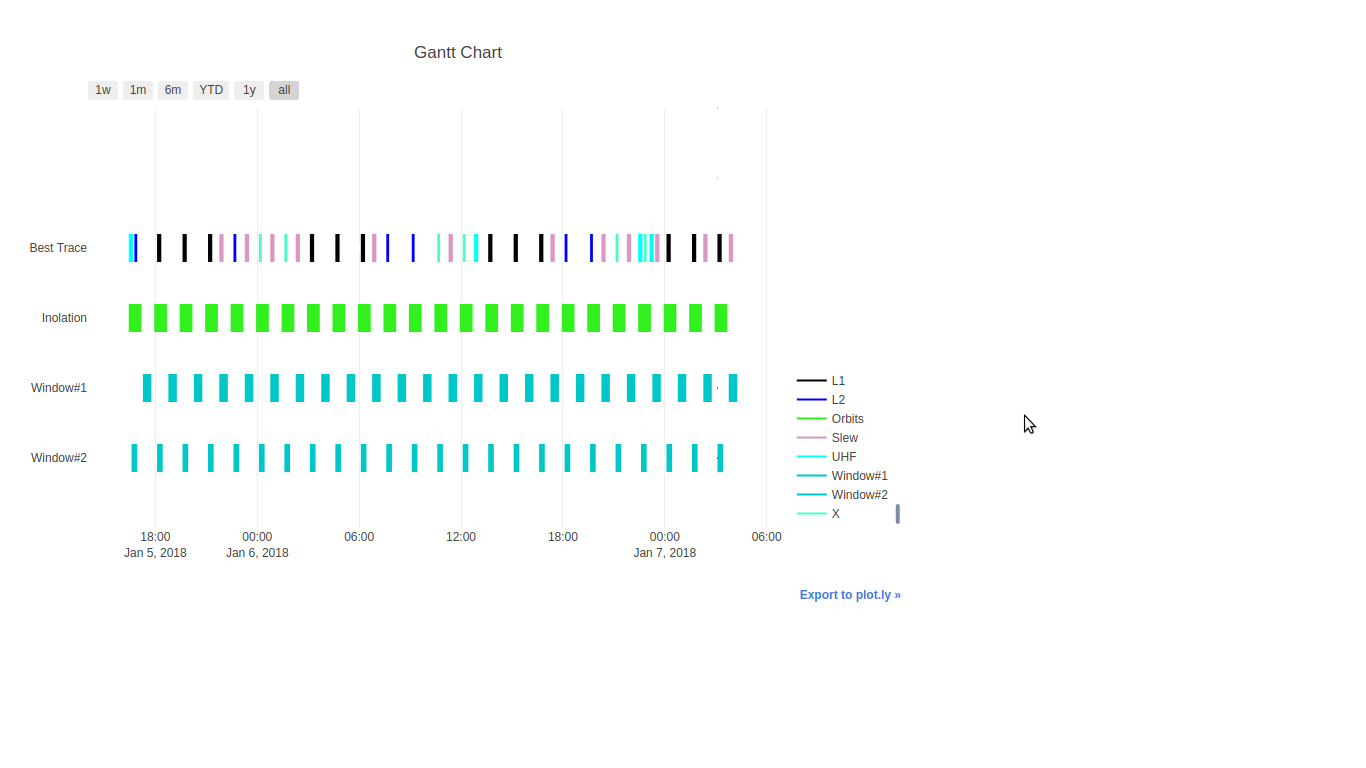
\includegraphics[width=\textwidth]{graphics/gantt.png}
	\caption{Graphical representation of the \gls{cora} schedule}
	\label{fig:gantt}
\end{figure}
The chart will be produced even if the robustness verification fails to accept the schedule. The user will therefore have acces to all of the charts throughout the iteration. By doing so, the user may analyse the charts to better figure out if the want to accept the schedules or if they want to adjust some of the payloads or parameters themselves.

\subsection{Queries}\label{sec:queries}
In order to verify the generated schedule and output relevant data, we have included several queries which can be run in UPPAAL \gls{smc}. We want to verity that we do not fall below the battery threshold, and the payloads that are scheduled are actually executed. Additionally, we want to monitor different variables in order to present the user with all the relevant data we are able to extract.\\
When probability queries are run, this is always done by a confidence factor of $95\%$.

\subsubsection*{Verifying the Battery Capacity}
It is expected that battery usage in the \gls{smc} model differs from that in the \gls{cora} model as they use two different battery models, Ideal and \gls{kibam}. The usage may also vary because of the possible difference in time usage that the individual payloads takes to complete. The time it takes to complete one payload in \gls{cora} are constant but in \gls{smc}it may vary, as we want to model the uncertainty.

We expect that we will use more energy in the \gls{smc} model because \gls{kibam} under estimates the energy consumption whereas the model used in \gls{cora} will overestimate. The \gls{smc} model is also guaranteed to use the same amount, or less, time to complete a payload than \gls{cora}. This is due to \gls{cora} model using the worst case time when executing the payloads.
% impotant
\begin{equation} \label{eq:smca}
	Pr\; [<=ScheduleLength] \; (<>\; a\ <\ 0.1)
\end{equation}
Query \ref{eq:smca} will result in a probability that reflects the risk of the battery's available charge falling below $0.1$. We added this query as depletion of the available charge can result in scheduled payloads being skipped.

\begin{equation} \label{eq:smcb}
	Pr\; [<=ScheduleLength] \; (<>\; b\ <\ ((1-c)*C) * (ThresholdPercentage\ /\ 100)
\end{equation}

The query seen in query \ref{eq:smcb} results in the probability of the bound charge falling below the user specified threshold e.g. $40\%$ of the maximum. If this would occur, the nanosatellite would enter its safe mode. Because this may not occur query \ref{eq:smcb} has been included.

\begin{equation} \label{eq:smctotal}
	Pr\; [<=ScheduleLength] \; (<>\; b\ +\ a\ <\ C\ *\ (ThresholdPercentage\ /\ 100)
\end{equation}
Query \ref{eq:smctotal} is the third and last query that may be used to ensure the battery capacity does not fall below any threshold. This indicates that the sum of available and bound energy may not fall below the specified threshold in regards to the batteries total capacity.

All of these queries are relevant to verify that the battery will hold up. However, as it may take considerable time to run a probability query, as it is unpredictable how many simulations it will run, we have chosen to only include query \ref{eq:smctotal} in the script. This query is chosen above the others as it is ultimately the one describing the nanosatellites state of charge.

\subsubsection*{Verifying the Payload Order}
% impotant
\begin{equation} \label{eq:smc3}
	Pr\; [<=ScheduleLength] \; (<> \ skips \ !=\ 0)
\end{equation}
Query \ref{eq:smc3} are used for finding the probability of any scheduled payloads are not run. The reason for it not doing so may vary but it will often be as a result of a low battery level as a result of a more precise battery model, which over predicts the energy consumption, implemented in the \gls{smc} model.\\
This query does not give any of information about what went wrong, however it does say that the generated schedule does not hold completely.

% extra
\begin{equation} \label{eq:smc4}
	simulate\ 100 \; [<=ScheduleLength] \; \{active, \; Processor.Running\}
\end{equation}
Query \ref{eq:smc4} is used in conjunction with query \ref{eq:smc3}. This is just 100 simulations which will each represent one random trace. However in case any payloads were skipped during these simulations, it will be possible to find which was skipped at what time.\\
What \ref{eq:smc4} does, is indicating what payload is supposed to execute at what time, and whether or not it was.

As these queries support each other and query \ref{eq:smc4} is just a 100 simulations and therefore more predictable in the time it takes to complete, both will be included in the script.

\begin{figure}[H]%
	\centering
	\subfloat
	{{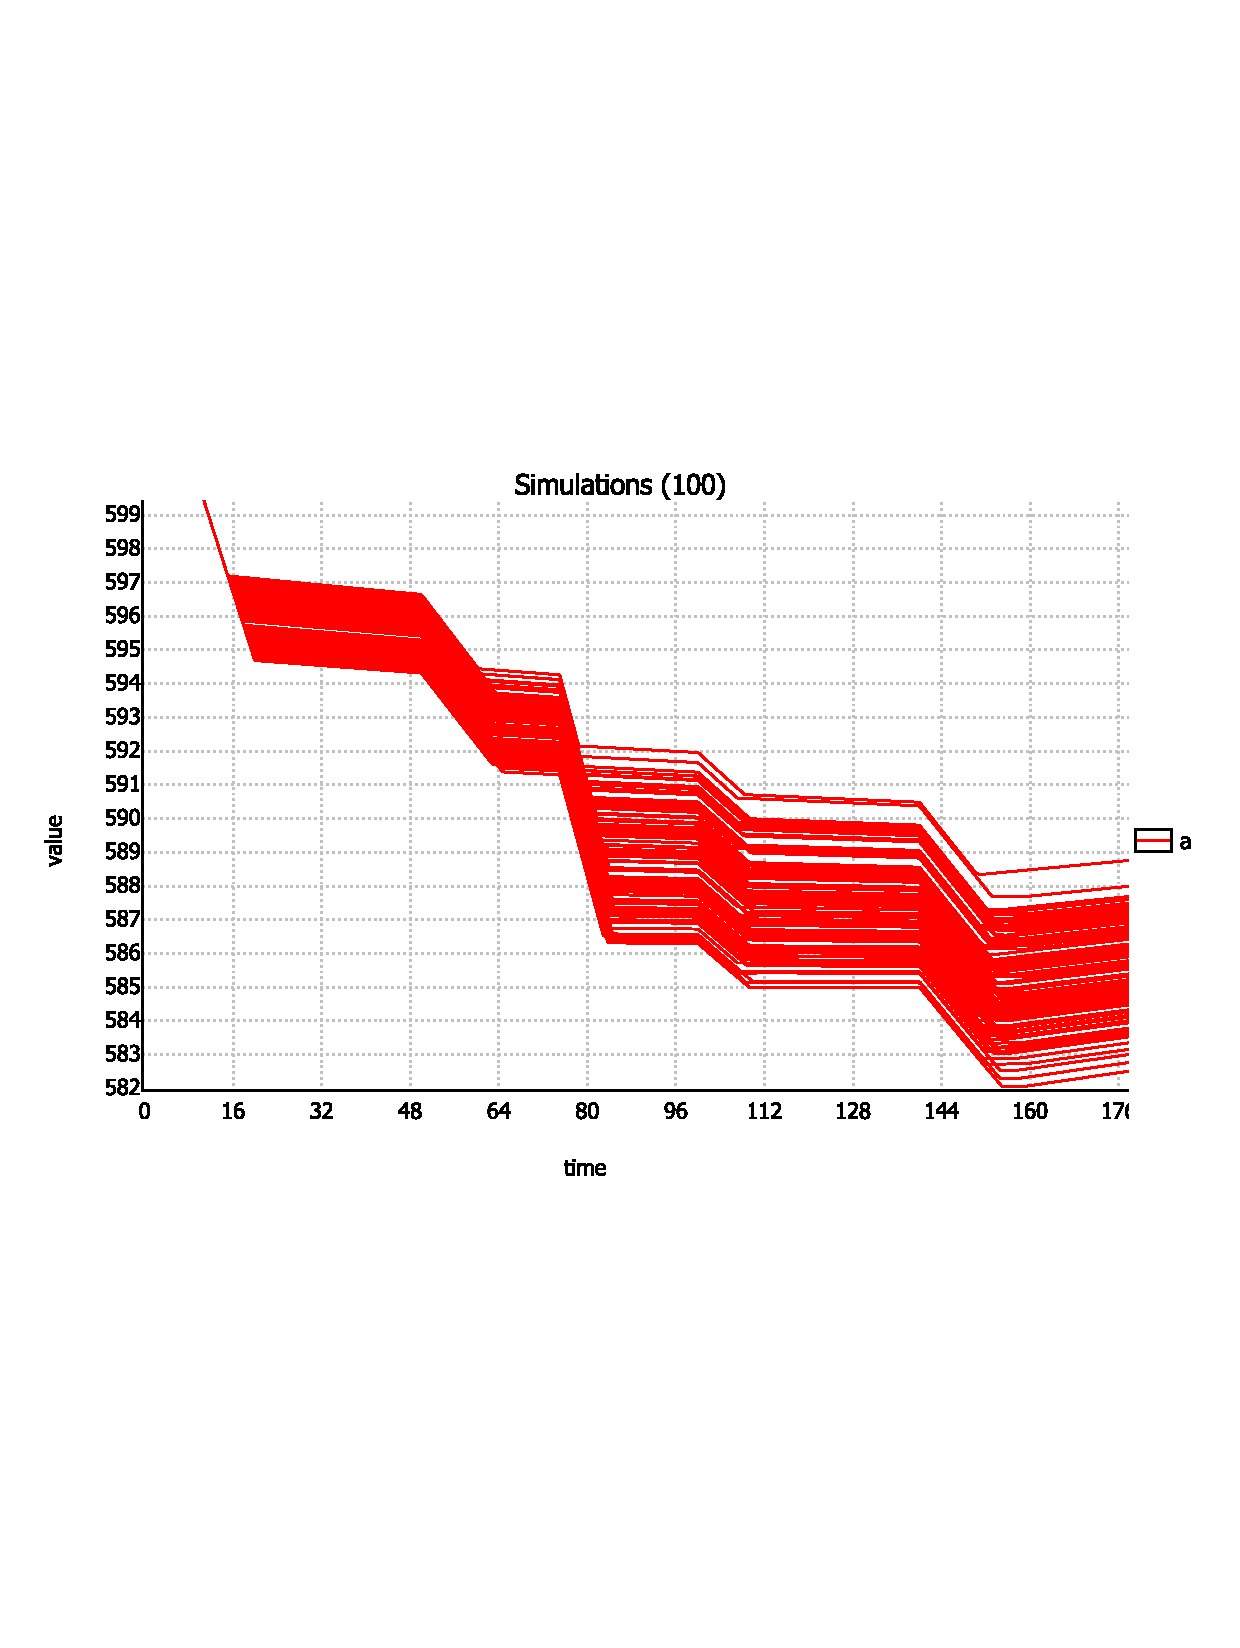
\includegraphics[width=7cm, trim={0 8cm 0 6cm},clip] {graphics/simulation_graphs/SimulationsA100.pdf} }}%
	\qquad
	\subfloat
	{{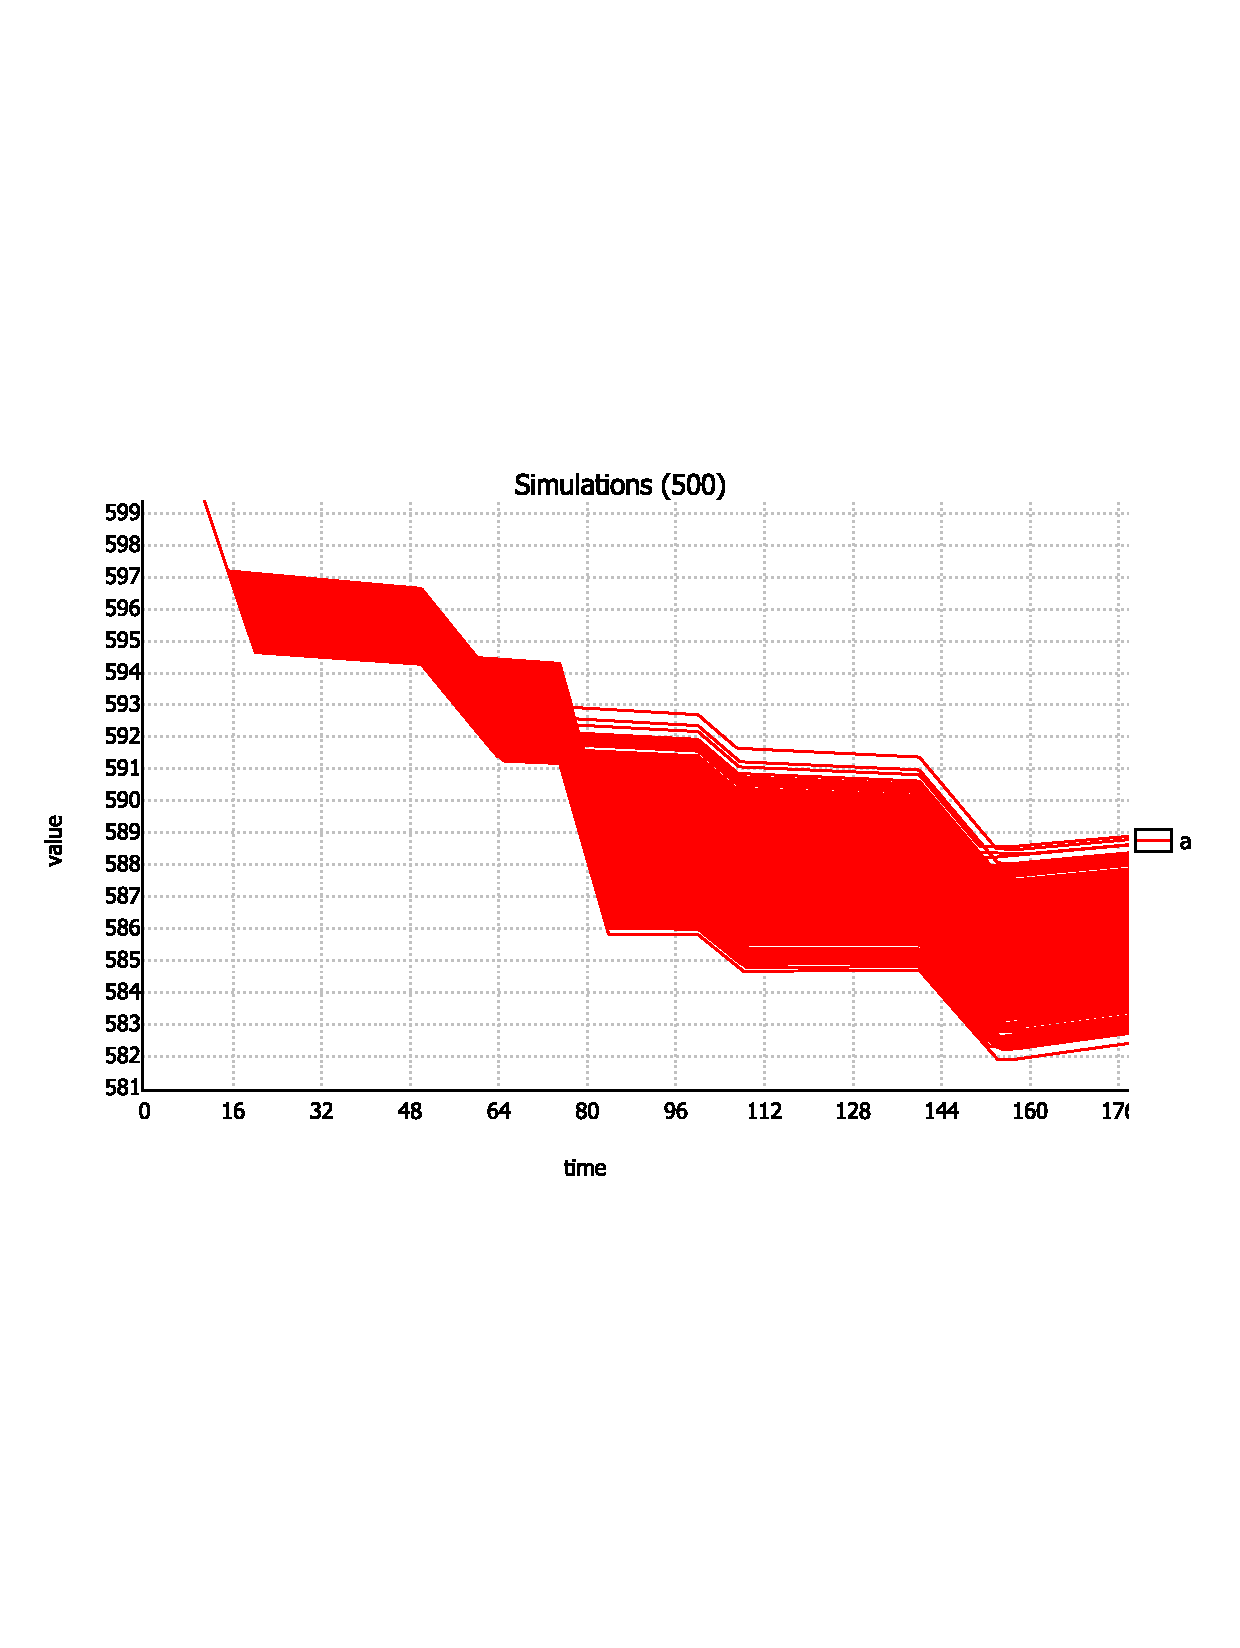
\includegraphics[width=7cm, trim={0 8cm 0 6cm},clip] {graphics/simulation_graphs/SimulationsA500.pdf} }}%
	\caption{100 simulations(left) versus 500 simulations(right) over available energy \textit{a} in smc}%
	\label{fig:sim_amount}%
\end{figure}
In query \ref{eq:smc4} it is specified that we want to run the simulation 100 times, the reason for this is that we consider 100 simulations is adequate to give a reasonable representation of the values range. In \cref{fig:sim_amount} we see two graphs, one where the simulation have been run 100 times and one where it have been run 500 times. It can there be seen that the lowest observed value of \textit{a} is similar in both graphs, $182$ in the one with 100 simulations and $181.9$ in the one with 500 simulations. And the highest value observed by the end of the simulations were $188.8$ versus $189$. In both cases the 500 simulations displays a wider range for the value, however the query running 100 simulations took $9$ seconds, whereas the one with 500 took $55$ seconds.\\
With the small differences to the final output and the large amount of time saved we conclude that running 100 simulations will give an acceptable range in short time. Therefore we will use 100 simulations for all queries of the type simulation.

\subsubsection*{Other Information}
\begin{equation} \label{eq:smc5}
	simulate\ 100 \; [<=\ ScheduleLength]\; \{ a,\ b\}
\end{equation}
Query \ref{eq:smc5} provides two time series that reflects the two wells of the battery, a and b. This is useful for the user as they might want to discard the schedule if it uses more energy than what they are comfortable with. Even if we do not go below the threshold, it may be to expensive to execute the schedule. 

% extra
\begin{equation} \label{eq:smc6}
	E \; [<=\ ScheduleLength;\ 100]\; ( max:\ earnings)
\end{equation}
Query \ref{eq:smc6} finds the accumulated profit for the schedule. We will not judge a schedule based on this value, we will let the user decide if it is acceptable, however the schedule is generated to maximize this value, see \myref{sec:cora}, and should therefore be viable. The profit is an abstract variable and we will not be able tell whether or not it is satisfactory.

The three last queries, \ref{eq:smc4}, \ref{eq:smc5}, and \ref{eq:smc6}, are tested with simulations. The simulations are great for giving the user insight in the behaviour of the nanosatellite when executing the schedule. \\
It does however not set any guarantees for the correctness or robustness of the schedule as it only displays the result of the path taken during each of the simulations.

